\documentclass[openany]{article}
\usepackage{float}
% Language setting
% Replace `english' with e.g. `spanish' to change the document language
\usepackage[spanish]{babel}
\usepackage{rotating}

% Set page size and margins
% Replace `letterpaper' with `a4paper' for UK/EU standard size
\usepackage[letterpaper,top=2cm,bottom=2cm,left=3cm,right=3cm,marginparwidth=1.75cm]{geometry}

% Useful packages
\usepackage{amsmath}
\usepackage{graphicx}
\usepackage[colorlinks=true, allcolors=blue]{hyperref}
\usepackage{array} % required for text wrapping in tables


\title{Memoria de la Práctica 3}

\begin{document}

\maketitle
\textbf{Integrantes del grupo}

\begin{itemize}
\item
  Carmen Chunyin Fernández Núñez
\item
  Pablo García Guijosa
\item
  Marta Xiaoyang Moraga Hernández
\item
  Jesús Navarrete Caparrós
\end{itemize}

\section{Índice}\label{uxedndice}

\hyperref[uxedndice]{\textbf{Índice}}

\hyperref[intro]{\textbf{Descripción 2}}

\hyperref[plan]{\textbf{Planificación 2}}

\hyperref[ana]{\textbf{Análisis de pruebas 3}}

\hyperref[dis]{\textbf{Diseño de pruebas 4}}

\hyperref[test]{\textbf{Implementación de los tests 5}}

\hyperref[results]{\textbf{Resultados tests 13}}

\pagebreak

 
\section{Descripcion}\label{intro}
Esta práctica ha consistido en diseñar e implementar una serie de tests, relativos a la funcionalidad del modelo de la aplicación creada para la práctica 2. Muchos no han requerido cambios al modelo subyacente, aunque algunas funcionalidades sí han requerido modificaciones, para lograr que su funcionalidad satisfaga las especificaciones de los tests propuestos.
\newline

Estos tests comprueban el correcto funcionamiento del modelo, tanto de las funcionalidades más simples (como añadir un empleado o departamento por sí solos), como operaciones más complejas (como añadir empleados o departamentos con datos iguales a otros ya añadidos, o eliminar bloques de departamentos y empleados anidados).
\newline

Además, se ha decidido modificar un comportamiento del modelo que en un principio considerábamos como válido, pero que actualmente hemos decidido modificar. Se trata de la posibilidad de que un empleado o departamento, de los mismos datos, pueda pertenecer a más de un departamento a la vez. En la versión que se entrega en esta práctica, si se intenta añadir a otro departamento un empleado o departamento con los mismos datos que otro que ya se encuentra en un departamento, lo único que se producirá es que el empleado (o departamento) cambiará a pertenecer sólamente al nuevo departamento donde se ha añadido, y no a los dos.


\section{Planificación de las pruebas del sistema} \label{plan}

Las pruebas ideadas para comprobar el funcionamiento de la aplicación son las siguientes:

\begin{enumerate}
    \item Añadir empleado a empleado
    \item Añadir departamento a departamento
    \item Añadir empleado de mismos datos en varios departamentos
    \item Añadir departamento de mismos datos en varios departamentos
    \item Añadir departamento a empleado
    \item Añadir empleado a departamento
    \item Añadir departamento a sí mismo
    \item Añadir empleado o departamento con datos parciales
    \item Añadir empleado fuera de departamento
    \item Eliminar elemento
    \item Eliminar bloque completo
    \item Eliminar con nada seleccionado
    \item Eliminar bloque elimina bien lo de dentro
\end{enumerate}


\pagebreak
\section{Análisis de pruebas}\label{ana}

\begin{table}[H]
    \centering
    \begin{tabular}{|>{\raggedright\arraybackslash}p{0.33\linewidth}|>{\raggedright\arraybackslash}p{0.33\linewidth}|>{\raggedright\arraybackslash}p{0.33\linewidth}|} \hline 
        \textbf{Elemento a probar} & \textbf{Condiciones} & \textbf{Datos requeridos}\\ \hline 
        Añadir empleado a empleado &  Tener 1 empleado creado& Contenido de sus arrays “elementos” respectivos después de intentar realizar la acción\\ \hline
        Añadir departamento a si mismo &  Tener 1 departamento creado& Contenido de sus arrays “elementos” respectivos después de intentar realizar la acción\\ \hline 
        Añadir departamento a departamento &  Tener 1 departamento creado& Contenido de sus arrays “elementos” respectivos después de intentar realizar la acción\\ \hline 
        Añadir empleado de mismos datos en varios departamentos &  Tener varios departamentos creados& Contenido de sus arrays “elementos” respectivos después de intentar realizar la acción\\ \hline 
        Añadir departamento de mismos datos en varios departamentos &  Tener varios departamentos creados& Contenido de sus arrays “elementos” respectivos después de intentar realizar la acción\\ \hline 
        Añadir departamento a empleado &  Tener 1 empleado creado& Contenido de sus arrays “elementos” respectivos después de intentar realizar la acción\\ \hline 
        Añadir empleado a departamento &  Tener 1 departamento creado& Contenido de sus arrays “elementos” respectivos después de intentar realizar la acción\\ \hline 
        Añadir empleado o departamento con datos parciales &  ---& ---\\ \hline 
        Añadir empleado fuera de departamento &  ---& ---\\ \hline 
        Eliminar elemento &  Tener creado al menos 1 elemento& Contenido de sus arrays “elementos” respectivos después de intentar realizar la acción\\ \hline 
        Eliminar bloque completo &  Tener creado al menos 1 departamento que, a su vez, tiene agregado como mínimo 1 departamento o 1 empleado& Contenido de sus arrays “elementos” respectivos después de intentar realizar la acción\\ \hline 
        Eliminar con nada seleccionado &  ---& ---\\ \hline 
        Eliminar bloque elimina bien lo de dentro &  Tener creado al menos 1 departamento que, a su vez, tiene agregado como mínimo 1 departamento o 1 empleado& Contenido de sus arrays “elementos” respectivos después de intentar realizar la acción\\ \hline
    \end{tabular}
    \caption{Análisis}
    \label{tab:analisis}
\end{table}
\pagebreak
\newgeometry{left=2cm,bottom=2cm,top=0.3cm}
\section{Diseño de pruebas}\label{dis}
\begin{table}[H]
    \centering
    \begin{tabular}{|>{\raggedright\arraybackslash}p{0.15\linewidth}|>{\raggedright\arraybackslash}p{0.25\linewidth}|>{\raggedright\arraybackslash}p{0.25\linewidth}|>{\raggedright\arraybackslash}p{0.35\linewidth}|} \hline 
        \textbf{Casos de prueba} & \textbf{Entornos de prueba} & \textbf{Datos de prueba} & \textbf{Trazabilidad}\\ \hline 
         Añadir empleado a empleado&  Ejecución normal del programa. No necesita herramientas adicionales&  Elemento Empleado al que se le intenta añadir un empleado, dentro de “elementos”&Aparece un nuevo error de tipo "UnimplementedError"\\ \hline 
         Añadir departamento a departamento&  Ejecución normal del programa. No necesita herramientas adicionales&  Elemento Departamento al que se le intenta añadir un departamento, dentro de “elementos”&“elementos” del departamento contiene un nuevo departamento, cuyo padre es el departamento donde queríamos incluirlo\\ \hline 
         Añadir empleado de mismos datos en varios departamentos&  Ejecución normal del programa. No necesita herramientas adicionales&  Elementos Departamento a los que se le intenta añadir un empleado, dentro de “elementos”&“elementos” del primer departamento ahora no contiene al empleado, mientras que “elementos” del segundo departamento ahora sí lo contiene\\ \hline 
         Añadir departamento de mismos datos en varios departamentos&  Ejecución normal del programa. No necesita herramientas adicionales&  Elementos Departamento a los que se le intenta añadir un departamento, dentro de “elementos”&“elementos” del primer departamento ahora no contiene al departamento, mientras que “elementos” del segundo departamento ahora sí lo contiene\\ \hline 
         Añadir departamento a empleado&  Ejecución normal del programa. No necesita herramientas adicionales&  Elemento Empleado al que se le intenta añadir un empleado, dentro de “elementos”&Aparece un nuevo error de tipo "UnimplementedError"\\ \hline 
         Añadir empleado a departamento&  Ejecución normal del programa. No necesita herramientas adicionales&  Elemento Departamento al que se le intenta añadir un empleado, dentro de “elementos”&“elementos” contiene un nuevo empleado, cuyo padre es el departamento donde queríamos incluirlo\\ \hline 
         Añadir empleado o departamento con datos parciales&  Ejecución normal del programa. No necesita herramientas adicionales&  Elemento Empleado o Elemento Departamento al que se le intenta añadir al sistema sin todos los campos llenos&Los elementos incompletos no estarán contenidos en el array de elementos del director\\ \hline 
         Añadir empleado fuera de departamento&  Ejecución normal del programa. No necesita herramientas adicionales&  Añadir un Elemento Empleado al sistema sin tener asociado ningún Elemento Departamento&“elementos” contiene un empleado que no tiene asociado ningún padre\\ \hline 
         Eliminar elemento&  Ejecución normal del programa. No necesita herramientas adicionales&  Eliminar un Elemento del sistema&El elemento eliminado no se encontrará en el array\\ \hline 
         Eliminar bloque completo&  Ejecución normal del programa. No necesita herramientas adicionales&Eliminar un Elemento Departamento que tenga subdepartamentos y/o empleados&Los elementos eliminados no estarán contenidos en el array de elementos del director\\ \hline 
         Eliminar con nada seleccionado&  Ejecución normal del programa. No necesita herramientas adicionales&  Intentar eliminar sin seleccionar ningún elemento&Ningún elemento se verá modificado, todos los elementos originales estarán contenidos en el array del director\\ \hline 
         Eliminar bloque elimina bien lo de dentro&  Ejecución normal del programa. No necesita herramientas adicionales&  Eliminar todos los “elementos” de todos los Departamentos y Empleados del bloque seleccionado&Verificar que los elementos fuera del bloque seleccionado no se ven afectados y que todos los elementos dentro del bloque se eliminan correctamente\\ \hline
    \end{tabular}
    \caption{Diseño}
    \label{tab:my_label}
\end{table}
\restoregeometry
\pagebreak
\section{Implementación de los test}\label{test}

En esta sección, se van a explicar las modificaciones que se han tenido
que realizar sobre el código para que las funcionalidades probadas a
partir de los test estuviesen implementadas correctamente.

\begin{enumerate}
\def\labelenumi{\arabic{enumi}.}
\item
  Añadir departamento a departamento
\end{enumerate}

\begin{quote}
Se ha tenido que modificar la función addElementoEmpresa(ElementoEmpresa
elemento) de la clase Departamento. Pues no se modifica el Departamento
Superior asociado al elemento que añadimos a la lista de elementos
empresa.

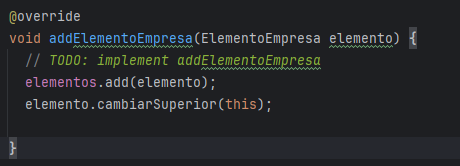
\includegraphics{imagenes/test2.png}
\end{quote}

\begin{enumerate}
\def\labelenumi{\arabic{enumi}.}
\setcounter{enumi}{1}
\item
  Añadir empleado a departamento
\end{enumerate}

\begin{quote}
Lo explicado en el punto anterior también ha sido aplicado a la clase
Empleado, además de implementar la función cambiarSuperior(), pues no
estaba implementada.

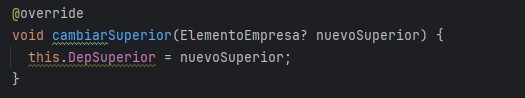
\includegraphics{imagenes/test6.png}
\end{quote}

\begin{enumerate}
\def\labelenumi{\arabic{enumi}.}
\setcounter{enumi}{2}
\item
  Añadir departamento/empleado de mismos datos en varios departamentos
\end{enumerate}

\begin{quote}
Esta funcionalidad se enfoca desde el hecho de que no se pueden añadir
el mismo empleado/departamento en dos departamentos diferentes, por ello
al añadirlos a un departamento, si ya pertenecían a otro, se modificará
el superior del elemento añadido y se eliminará del antiguo superior.

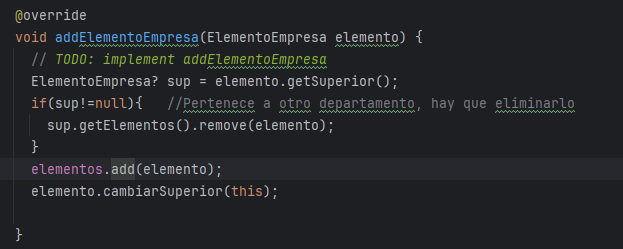
\includegraphics{imagenes/test4.png}
\end{quote}

\begin{enumerate}
\def\labelenumi{\arabic{enumi}.}
\setcounter{enumi}{3}
\item
  Añadir un departamento a sí mismo
\end{enumerate}

\begin{quote}
Si un departamento intenta añadirse a su propia lista de departamentos,
deberá lanzarse un error. Para ello, hemos modificado la función
cambiarSuperior, para que compruebe si el elemento que se intenta añadir
es uno mismo. Además de cambiar el orden de las operaciones dentro de la
función addElementoEmpresa.

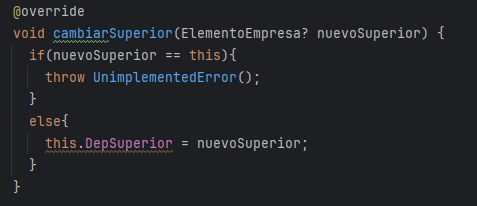
\includegraphics{imagenes/test_extra.png}

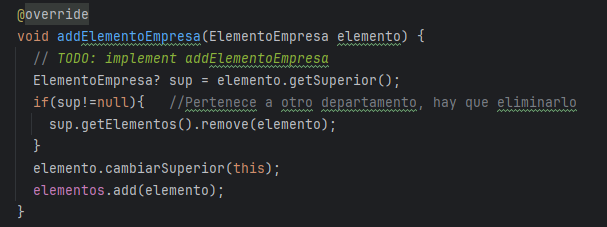
\includegraphics{imagenes/test_extra2.png}
\end{quote}

\begin{enumerate}
\def\labelenumi{\arabic{enumi}.}
\setcounter{enumi}{4}
\item
  La posibilidad de añadir un elemento empresa directamente con
  director.
\end{enumerate}

\begin{quote}
En nuestro modelo inicial, se ofrecía poder añadir un departamento o un
empleado utilizando sus datos con las funciones de addDepartamento y
addEmpleado, respectivamente, que se encargan de crear el elemento
indicado. Sin embargo, el director carecía de un addElementoEmpresa para
añadir elementos ya creados, que ahora añadimos. Puesto que queremos
evitar que se añadan a la empresa elementos sin los datos adecuados, se
añaden comprobaciones similares a las que tenían addDepartamento y
addEmpleado.
\end{quote}

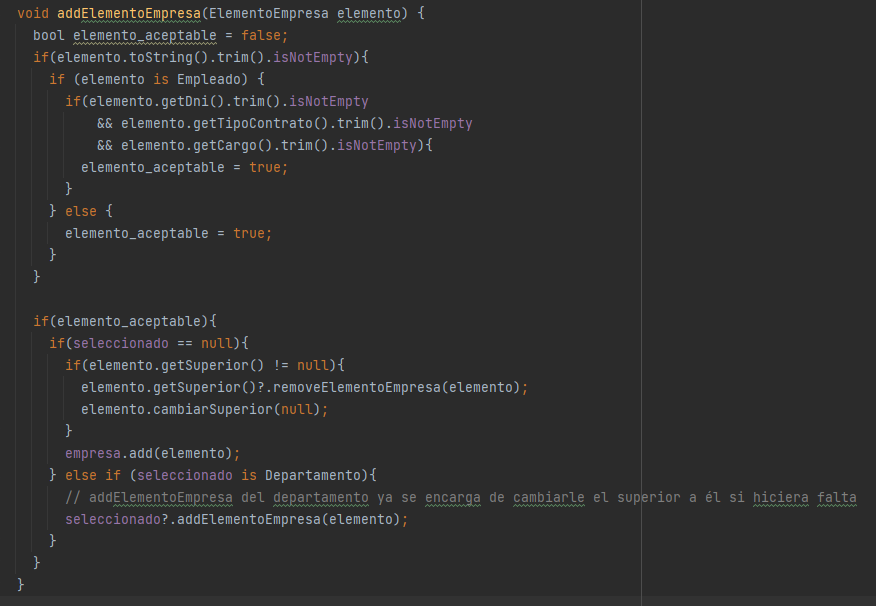
\includegraphics[width=6.26772in,height=4.33333in]{imagenes/addElementoEmpresa.png}

\pagebreak

Para facilitar la corrección, incluimos el código de los test.

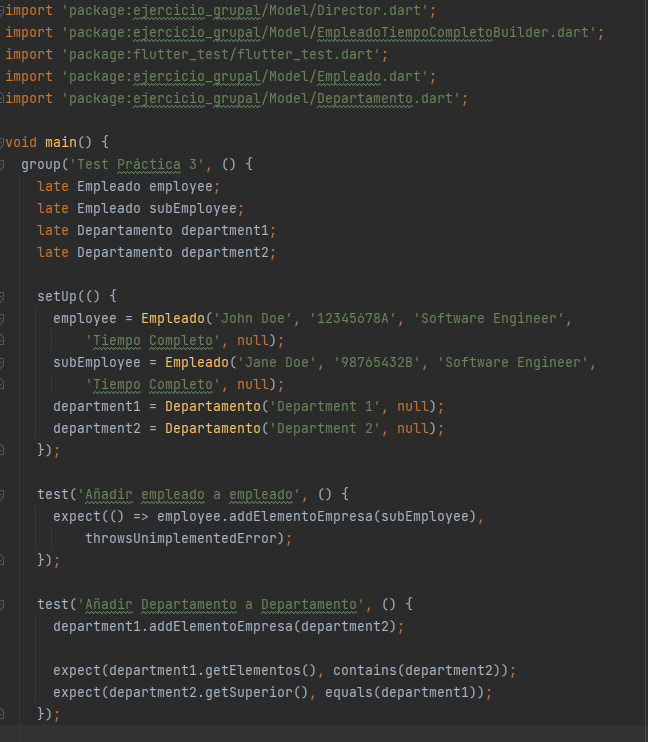
\includegraphics[width=6.26772in,height=7.18056in]{imagenes/testGrupo1.png}

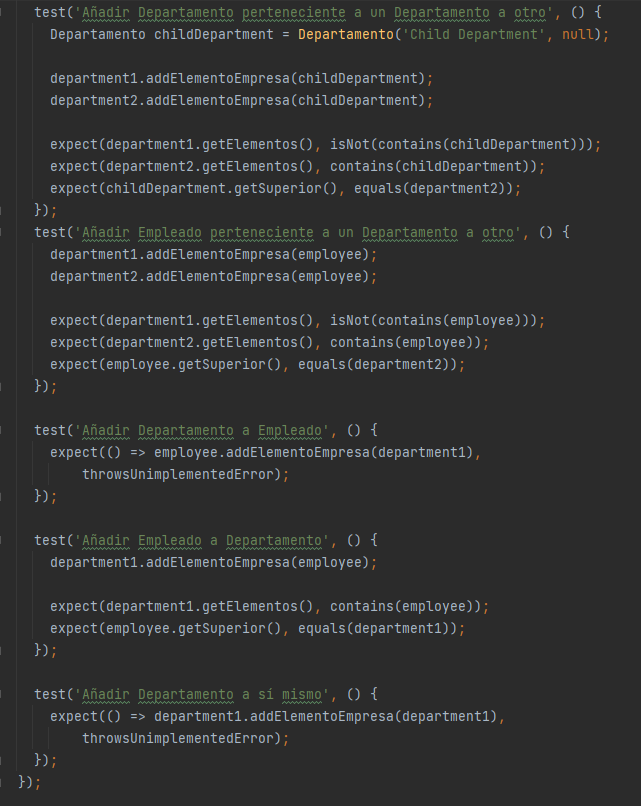
\includegraphics[width=6.26772in,height=7.875in]{imagenes/testGrupo1part2.png}

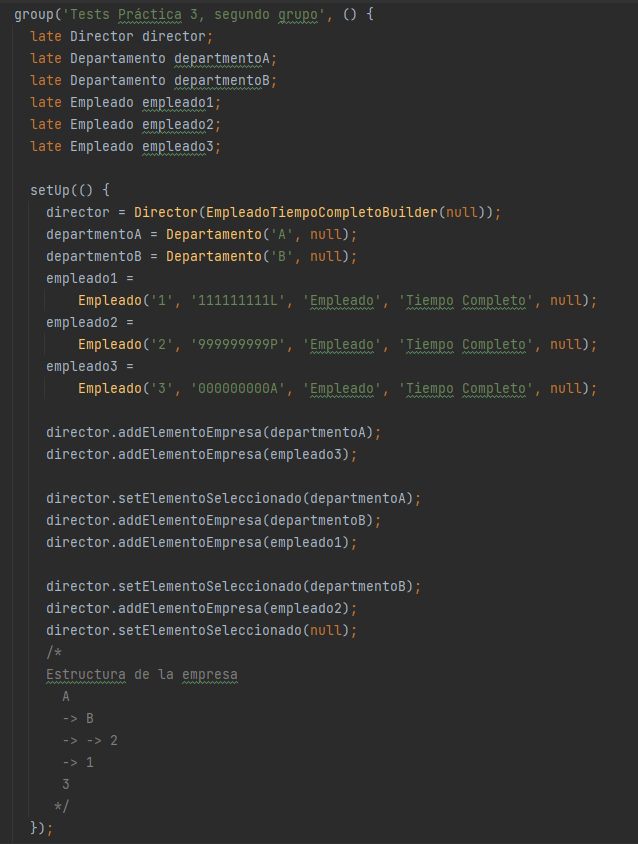
\includegraphics[width=6.26772in,height=8.29167in]{imagenes/testGrupo2.png}

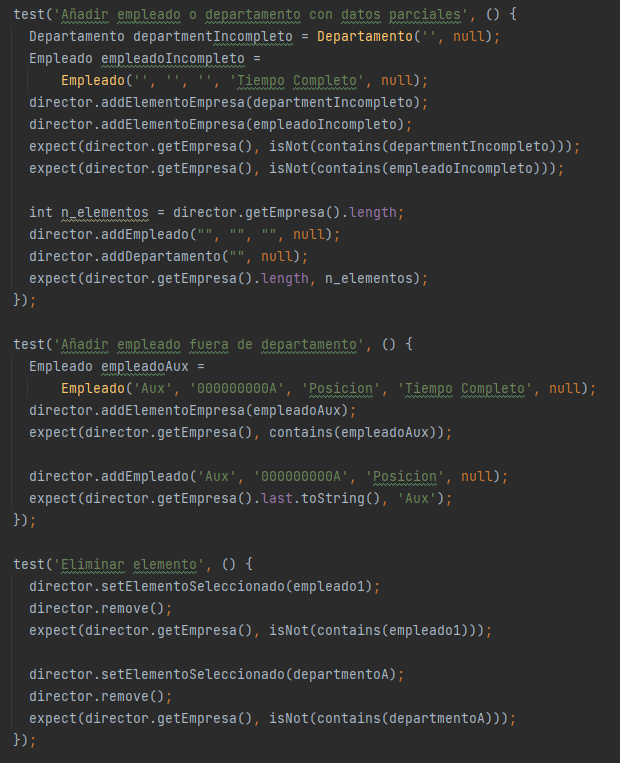
\includegraphics[width=6.26772in,height=7.70833in]{imagenes/testGrupo2part2.png}

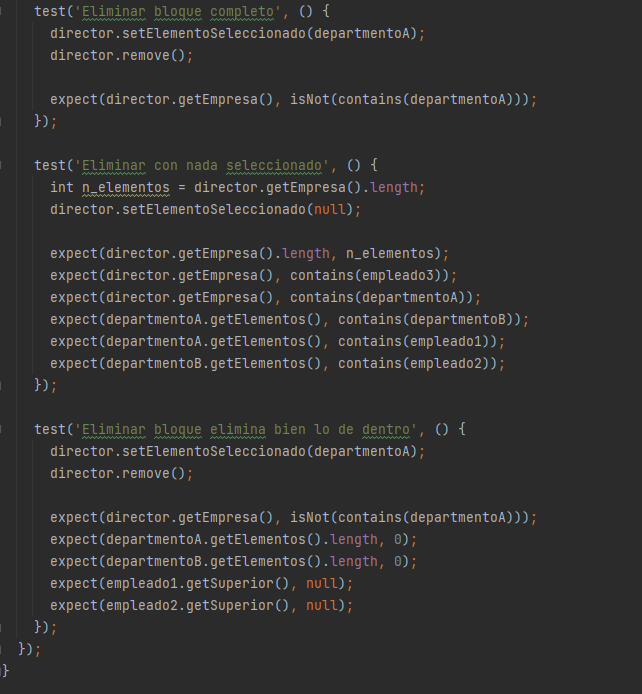
\includegraphics[width=6.26772in,height=6.77778in]{imagenes/testGrupo2part3.png}

\pagebreak
\section{Resultados tests} \label{results}
El resultado de los tests:\newline


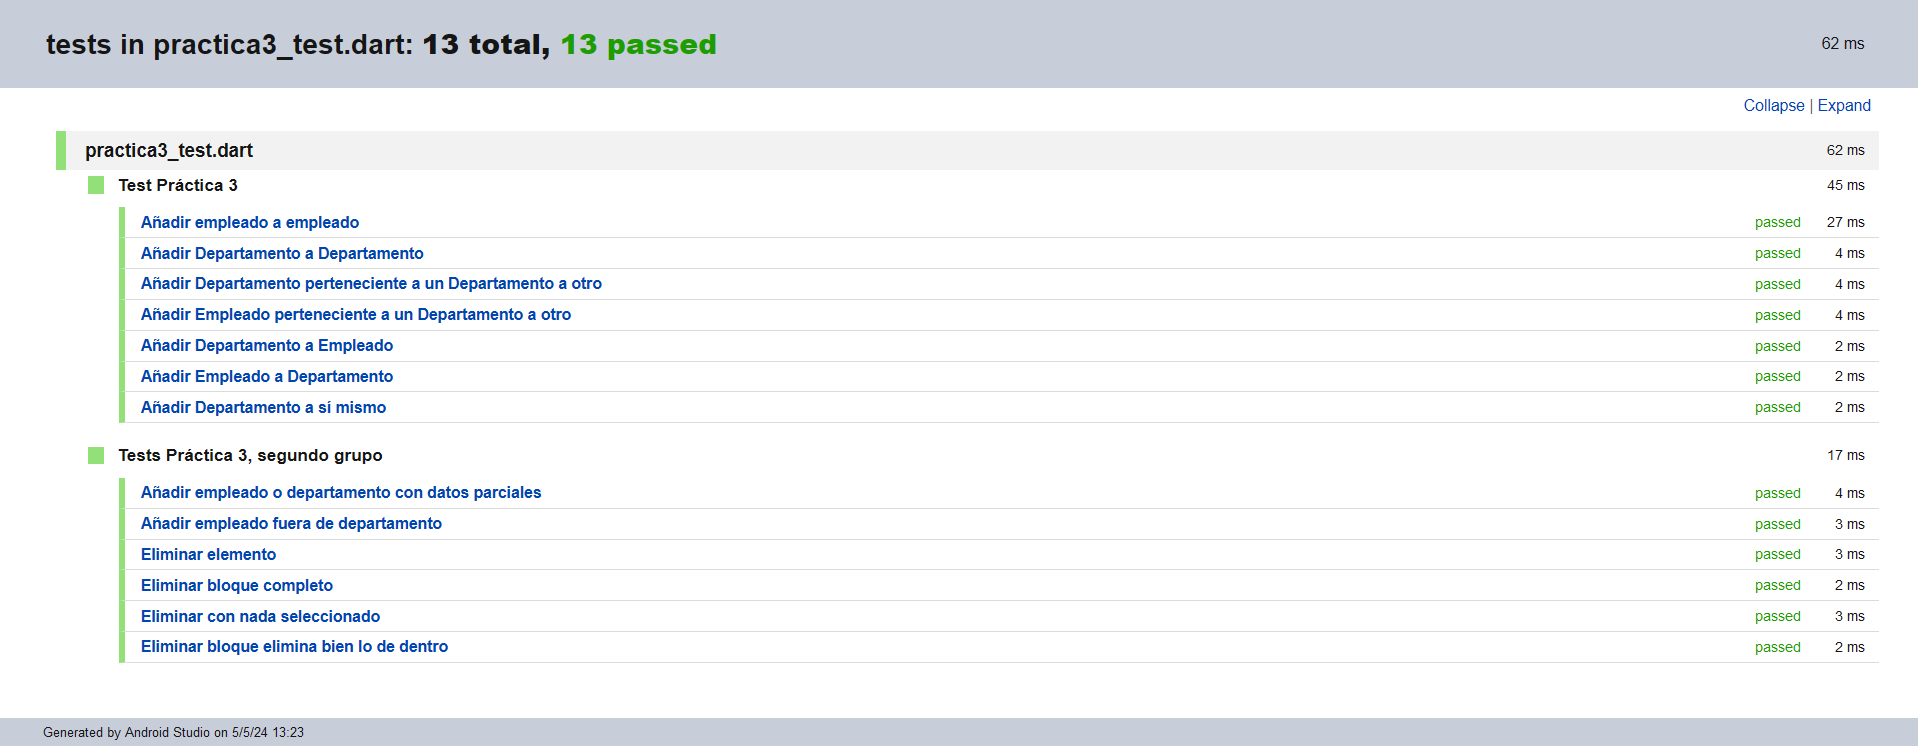
\includegraphics[width=6.26772in,height=2.44444in]{imagenes/testPasados.png}

\end{document}

